\documentclass[main.tex]{subfiles}

\begin{document}

\section{Electromagnetism}

\subsection{Magnetism} \label{24h7hD}

A magnet is a material that exerts a magnetic force on other magnets\footnote{For an example of the power of the magnetic force, see \textit{Breaking Bad} (\href{https://youtu.be/gzCXowhks80?t=4}{click here}).}. That's why you can stick magnets to your fridge. The \gls{magnetic pole} is the part of a magnet that exerts the strongest force on other magnets or magnetic material. This universe only allows the existence of a \gls{magnetic dipole}, which means that a magnet has two, and only two, poles: the \gls{north pole} (N) and \gls{south pole} (S). When two magnets are placed near each other, opposite poles attract, and like poles repel.

\begin{center}
    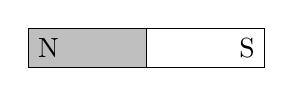
\begin{tikzpicture}
        \draw[fill=lightgray] (0,0) node[above right]{N} rectangle ++(1.5,0.5);
        \draw (3,0) node[above left] {S} rectangle ++(-1.5,0.5);
    \end{tikzpicture}
    \captionsetup{type=figure,margin=1in}
    \captionof{figure}{A bar magnet.}
\end{center}


What happens if you cut a magnet in half? You get two magnets, each with north and south poles. If you cut one of those magnets in half, you get the same bifurcation. You can continue this cutting-in-half of magnets until you reach the level of the atom, at which point you still have north and south poles! Thus, it is said, \textit{magnetism can be traced to the subatomic level}.

\begin{center}
    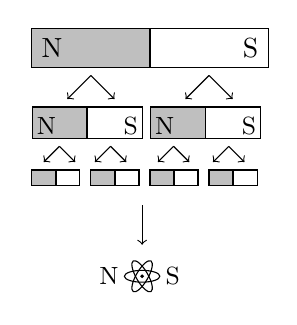
\begin{tikzpicture}[atom/.style = {circle,color=white, minimum size=#1,
    append after command={%
      \pgfextra{ 
        \foreach \ang in {0,120,240}
        \draw[rotate around={\ang:(0,0)}] (\tikzlastnode.center) ellipse (0.45*#1 and 0.15*#1); 
        \fill (\tikzlastnode.center) circle (0.05*#1);
      }
    }
  }
] %Source: https://tex.stackexchange.com/questions/349960/how-to-draw-a-symbol-on-a-tikz-node-that-can-be-reused
        \draw[fill=lightgray] (0,0) node[above right]{N} rectangle ++(1.5,0.5);
        \draw (3,0) node[above left] {S} rectangle ++(-1.5,0.5);
        \draw[->] (0.75,-0.1) -- ++(-0.3,-0.3); 
        \draw[->] (0.75,-0.1) -- ++(0.3,-0.3);
        \draw[fill=lightgray] (0.01,-0.9) node[above right=-2pt]{\small N} rectangle ++(0.7,0.4);
        \draw (1.4,-0.9) node[above left=-2pt] {\small S} rectangle ++(-0.7,0.4);
        \begin{scope}[xshift=1.5cm]
            \draw[->] (0.75,-0.1) -- ++(-0.3,-0.3); 
            \draw[->] (0.75,-0.1) -- ++(0.3,-0.3);
            \draw[fill=lightgray] (0.01,-0.9) node[above right=-2pt]{\small N} rectangle ++(0.7,0.4);
            \draw (1.4,-0.9) node[above left=-2pt] {\small S} rectangle ++(-0.7,0.4);
        \end{scope}
        \begin{scope}[xshift=0.35cm,yshift=-1cm]
            \draw[->] (0,0) -- ++(-0.2,-0.2); 
            \draw[->] (0,0) -- ++(0.2,-0.2);
        \end{scope}
        \begin{scope}[xshift=1cm,yshift=-1cm]
            \draw[->] (0,0) -- ++(-0.2,-0.2); 
            \draw[->] (0,0) -- ++(0.2,-0.2);
        \end{scope}
        \begin{scope}[xshift=1.8cm,yshift=-1cm]
            \draw[->] (0,0) -- ++(-0.2,-0.2); 
            \draw[->] (0,0) -- ++(0.2,-0.2);
        \end{scope}
        \begin{scope}[xshift=2.5cm,yshift=-1cm]
            \draw[->] (0,0) -- ++(-0.2,-0.2); 
            \draw[->] (0,0) -- ++(0.2,-0.2);
        \end{scope}
        \begin{scope}[yshift=-1cm]
            \draw[fill=lightgray] (0,-0.5) rectangle ++(0.3,0.2);
            \draw (0.61,-0.5)  rectangle ++(-0.3,0.2);
        \end{scope}
        \begin{scope}[yshift=-1cm,xshift=0.75cm]
            \draw[fill=lightgray] (0,-0.5) rectangle ++(0.3,0.2);
            \draw (0.61,-0.5)  rectangle ++(-0.3,0.2);
        \end{scope}
        \begin{scope}[yshift=-1cm,xshift=1.5cm]
            \draw[fill=lightgray] (0,-0.5) rectangle ++(0.3,0.2);
            \draw (0.61,-0.5)  rectangle ++(-0.3,0.2);
        \end{scope}
        \begin{scope}[yshift=-1cm,xshift=2.25cm]
            \draw[fill=lightgray] (0,-0.5) rectangle ++(0.3,0.2);
            \draw (0.61,-0.5)  rectangle ++(-0.3,0.2);
        \end{scope}
        \draw[->] (1.4,-1.75) -- ++(0,-0.5);
        \node[draw, atom=5mm] (C2) at (1.4,-2.65){};
        \node[left=5pt] at (1.4,-2.65){\small N};
        \node[right=5pt] at (1.4,-2.65){\small S};
    \end{tikzpicture}
    \captionsetup{type=figure,margin=1in}
    \captionof{figure}{Cutting a bar magnet in half, recursively, till you reach the atom.}
\end{center}

Magnets have a \gls{magnetic field}, which is a configuration of lines that indicate the direction and magnitude of the magnetic force. Magnetic field lines are invisible but can be visualized by sprinkling iron filings around a magnet. Magnetic field lines may also be mapped out using a compass. 

\vfill

\begin{center}
\begin{tikzpicture}
\def\lmag{1.8}  % length of magnet
\def\wmag{0.4}  % thickness of magnet
\def\nc{5}      % no. of lines = 2*\nc+1
\def\commandA{({90-asin(\lmag/(2*\r))})}
\def\commandB{({-270+asin(\lmag/(2*\r))})}

\begin{scope}
\coordinate (A) at (-\lmag/2,\wmag/2);
\coordinate (B) at (-\lmag/2,-\wmag/2);
\draw (A) rectangle ++(\lmag/2,-\wmag)node[midway]{S};
\draw[fill=lightgray](0,-\wmag/2) rectangle ++(\lmag/2,\wmag)node[midway]{N};

\clip (-5,-3) rectangle (5,3);
\foreach \r in {1,...,\nc}{
\draw[fLines]($(A)-(0,0.5*\r*\wmag/\nc)$) arc(({270-asin(\lmag/(2*\r))}):({-90+asin(\lmag/(2*\r))}):\r);
\draw[fLines]($(B)+(0,0.5*\r*\wmag/\nc)$) arc(\commandB:\commandA:\r); }
\draw[fLines] (-\lmag/2,0) -- ++(-6,0);
\draw[fLines] (\lmag/2,0) ++(6,0)--(\lmag/2,0);
\end{scope}
\end{tikzpicture}
\captionsetup{type=figure,margin=1in}
\captionof{figure}{A bar magnet and its magnetic field lines. A tiny magnet at a point on a magnetic field line will feel a magnetic force that is in the direction of the field.}
\end{center}

\vspace{1em}

A compass is a tiny magnet on a pivot. Like any ordinary magnet, the north pole of a compass points to the south pole of another magnet. Consider that a navigational compass points to Earth's north geographic\footnote{The prefix \textit{geo-} means ``earth,'' and \textit{geography} relates to the study of Earth's area and physical features.} pole. Thus you may pretend that Earth contains a giant magnet running through its core. Since the north magnetic pole of a compass points to Earth's north geographic pole, it follows that the \textit{north geographic} pole must be a \textit{south magnetic} pole. The same reasoning applies to the south geographic pole.

\begin{mdframed}[backgroundcolor=black!10]
\centering
    \textbf{The north geographic pole is a south magnetic pole.}
\end{mdframed}

\vspace{-1cm}

\begin{center}
\begin{tikzpicture}
    \node[rotate=23.5] at (4,0) {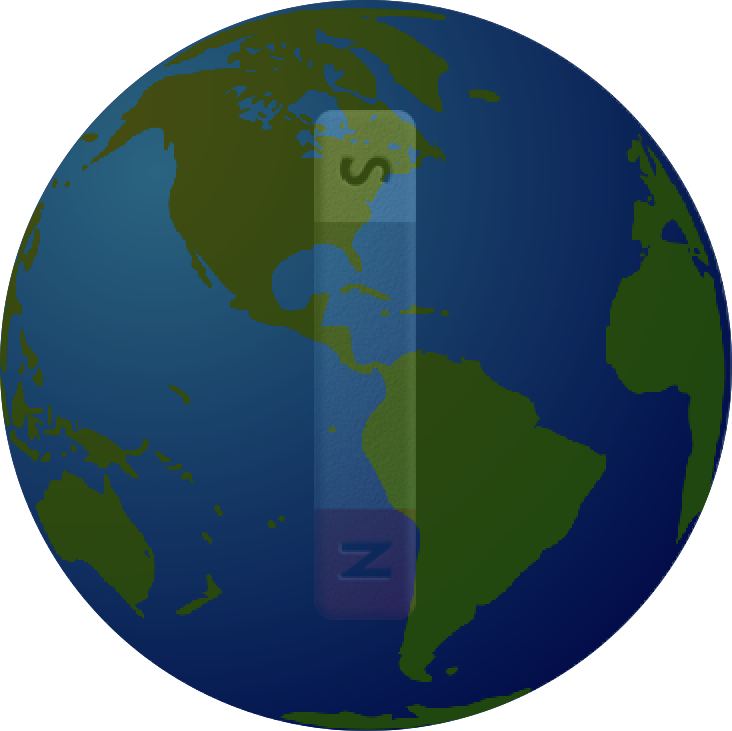
\includegraphics[width=5cm]{figures/Unit10_PhET_Earth.png}};
    \begin{scope}[rotate=-45,transform shape,yshift=8mm,xshift=-2mm]
        \draw (0,0) circle (1);
        \node[below] at (0,1) {N};
        \node[above] at (0,-1) {S};
        \node[left] at (1,0) {E};
        \node[right] at (-1,0) {W};
        \draw (-0.2,0) -- (0.2,0) -- (0,-0.6) -- (-0.2,0);
        \draw[fill=lightgray] (-0.2,0) -- (0.2,0) -- (0,0.6) -- (-0.2,0);
    \end{scope}
    \node at (0.35,-0.55) {compass};
\end{tikzpicture}
\vspace{-1cm}
\captionsetup{type=figure,margin=1in}
\captionof{figure}{Earth acting as a giant bar magnet. The south pole of this magnet lies in the northern hemisphere. Source: \texttt{PhET Simulation: Magnet and Compass} (\href{https://phet.colorado.edu/en/simulations/magnet-and-compass}{click here}).}
\end{center}

\vfill

\subsection*{\ref{24h7hD} Exercises}

\begin{exercise}
    Click the following link to watch ``The Big Bang Theory: Helium (Clip)'' by \texttt{TBS} on \texttt{YouTube} (\href{https://youtu.be/Q6Z0pCax9b8}{click here}). What is Sheldon talking about?
\end{exercise}

\begin{exercise}
    What does it mean that all magnets are magnetic \textit{dipoles}?
\end{exercise}

\begin{exercise}
    Where ever they look, physicists have failed to discover the presence of magnetic \textit{monopoles} in the universe. How many poles would a magnetic monopole have?
\end{exercise}

\begin{exercise}
    What are the labels for the poles of a bar magnet?
\end{exercise}


\begin{exercise}
    In your own words, describe what happens if you cut a magnet in half. If helpful, draw a picture.
\end{exercise}

\begin{exercise}
    What is a magnetic field?
\end{exercise}

\begin{exercise}
    Draw the magnetic field lines for the magnet shown below.

\begin{center}
    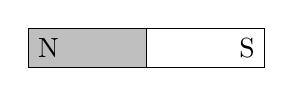
\begin{tikzpicture}
        \draw[fill=lightgray] (0,0) node[above right]{N} rectangle ++(1.5,0.5);
        \draw (3,0) node[above left] {S} rectangle ++(-1.5,0.5);
    \end{tikzpicture}
\end{center}
\end{exercise}

\begin{exercise}
    Click the link to access the \texttt{PhET Simulation: Magnet and Compass} (\href{https://phet.colorado.edu/en/simulations/magnet-and-compass}{click here}). Explore how a compass behaves around a bar magnet, and how Earth behaves as a giant bar magnet.
\end{exercise}

\begin{exercise}
    Explain why the north magnetic pole of a compass points towards geographic north. 
\end{exercise}

\begin{exercise}
    What type of magnetic pole is Earth's south geographic pole?
\end{exercise}

\begin{exercise}
    Sketch planet Earth and the magnetic field lines that surround it. (\textit{Hint}: Remember that you may pretend a giant bar magnet runs through the center of the planet.) 
\end{exercise}

\clearpage
\subsection{Electromagnetism} \label{okuZoJ}


Magnets are not the only things that create magnetic fields. Recall that electric current is electric charge that is in motion. Moving electric charges (electricity) are closely linked with magnetism. In fact, the study of electric and magnetic phenomena is called \gls{electromagnetism}. Here, we arrive at one of the core principles of electromagnetism:

\begin{mdframed}[backgroundcolor=black!10]
    \centering
    \textbf{Electric current generates a magnetic field.}
\end{mdframed}

%An \gls{electromagnet} is a device that uses electric current to make a magnetic field.


Electric current, which is mathematically represented as the rate at which electric charges flow, is measured in units of coulombs per second, or amperes (A). We focus on electric current that flows through wires. The convention is that current ($I$) flows opposite to the flow of electrons. For example, in a vertically oriented wire, if the electrons flow downwards, then current is defined as moving upwards.

\begin{mdframed}[backgroundcolor=black!10]
    \centering
    \textbf{The direction of current ($I$) is the direction opposite the flow of electrons.}
\end{mdframed}

Electric current flowing through a straight wire creates a unique, 3-dimensional magnetic field. Consider electrons flowing downwards through a vertical wire, as shown below. Current flows upwards. The magnetic field ($B$) beyond the wire has a circular shape. We can visualize this magnetic field using the \gls{right-hand rule}, which shows the direction of magnetic field outside wire. If your right thumb points in direction of current, then your fingers curl in direction of the magnetic field. 

\begin{center}
\begin{minipage}{0.3\textwidth}
\centering
    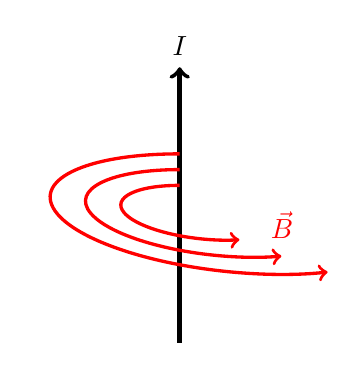
\begin{tikzpicture}
        \draw[ultra thick,->] (0,-2) -- ++(0,3.5) node[above] {$I$};
        \begin{scope}[rotate around x=50]
            \draw[red,very thick,->] (0,0) arc (90:280:1);
        \end{scope}
        \begin{scope}[yshift=2mm,rotate around x=50]
            \draw[red,very thick,->] (0,0) arc (90:283:1.6);
        \end{scope}
        \begin{scope}[yshift=4mm,rotate around x=50]
            \draw[red,very thick,->] (0,0) arc (90:286:2.2);
        \end{scope}
        \node[red] at (1.3,-0.5) {$\vec{B}$};
    \end{tikzpicture}
\end{minipage}%
\hspace{1em}
\begin{minipage}{0.3\textwidth}
    \centering
        
\includegraphics[width=3.6cm]{figures/Unit10_RightHandRule.jpeg}
\end{minipage}
    \captionsetup{type=figure,margin=1in}
    \captionof{figure}{An electric current ($I$) flowing upwards through a wire and the resulting magnetic field ($B$) surrounding the wire. The right-hand rule helps you visualize the magnetic field around the wire. \textbf{Art credit}: Ryan O.~(2023).}
    \label{H3bKoc}
\end{center}

% Video: \href{https://youtu.be/DDE3E5myE9s}{National MagLab: Right and Left Hand Rules}




Consider the plane of this page you are reading. Suppose a wire runs up the page. Due to the 3-dimensional shape of the magnetic field, the field will come \textit{out of the page} on the left side of the wire and go \textit{into the page} on the right. Try showing this phenomenon using the right-hand rule. 

\vspace{1em}

Let $\odot$ represent the magnetic field ($\vec{B}$) coming \textit{out} of the page and $\otimes$ represent going \textit{into} the page:


\begin{center}
    $\odot = $ out of the page\\
    $\otimes = $ into the page
\end{center}

\clearpage

Then we can symbolize the field around the wire as follows:

\begin{center}
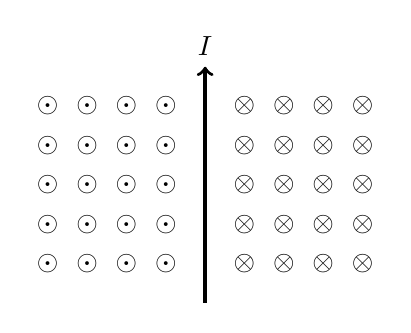
\begin{tikzpicture}
    \draw[very thick, ->] (0,0) -- ++(0,3) node[above] {$I$}; 
    \foreach \i in {0,0.5,...,1.5}
        \foreach \j in {0.5,1.0,...,2.5}
      {
        \begin{scope}[xshift=-2cm]
            \node at (\i,\j) {$\odot$};
        \end{scope}
        \begin{scope}[xshift=0.5cm]
            \node at (\i,\j) {$\otimes$};
        \end{scope}
      }
\end{tikzpicture}
\captionsetup{type=figure,margin=1in}
\captionof{figure}{To the left of the wire, magnetic field comes out of the page. To the right, it goes into the page. This is a 2-dimensional way of showing what is depicted in Figure \ref{H3bKoc}.}
\end{center}

\subsection*{\ref{okuZoJ} Exercises}

\begin{exercise}
    List two things that generate a magnetic field.
\end{exercise}

\begin{exercise}
    What is the relation between the direction of the flow of electrons through a wire and the direction of electric current?
\end{exercise}

\begin{exercise}
    Electrons flow rightwards through a horizontal wire. What is the direction of electric current through that wire?
\end{exercise}

\cyanhrule 

\vspace{1em}

\textbf{\ref{HBsxRL}--\ref{JE9nz0}}. Consider the electric current through a wire, as shown below.

\begin{center}
    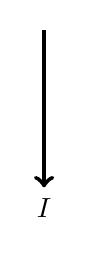
\begin{tikzpicture}
        \draw[ultra thick,->] (0,0) -- ++(0,-2) node[below] {$I$};
    \end{tikzpicture}
\end{center}

\begin{exercise} \label{HBsxRL}
    In which direction do the electrons through the wire flow?
\end{exercise}

\begin{exercise} \label{kCM6zG}
    Sketch some magnetic field lines surrounding the wire, in 3 dimensions. (\textit{Hint}: See Figure \ref{H3bKoc}, and use the right-hand rule.)
\end{exercise}

\begin{exercise} \label{hEl5WK}
    In two dimensions, using symbols $\odot$ and $\otimes$, draw the magnetic field going into and out of the page on either side of the wire.
\end{exercise}

\begin{exercise} \label{JE9nz0}
    Repeat sketches in Exercises \ref{kCM6zG} and \ref{hEl5WK} if the electrons through the wire flow to the left. 
\end{exercise}

\clearpage

\subsection{Calculating Magnetic Field Strength Outside a Straight Wire} \label{NErSiN}
The strength of the magnetic field varies as a function of distance from an electric current. The \textit{closer} you get to a current-carrying wire, the \textit{stronger} the magnetic field. Conversely, the farther get from the wire, the weaker the field. 

\begin{center}
    \begin{tikzpicture}
        \draw[ultra thick,->] (0,0) -- ++(0,3) node[above] {$I$};
        \draw[dashed] (0,2) -- ++(1,0) (0,1) -- ++(5,0); 
        \draw[fill=black] (1,2) circle (2pt) node[right=2pt] {$r_1$ (stronger field)};
        \draw[fill=black] (5,1) circle (2pt) node[right=2pt] {$r_2$ (weaker field)};
    \end{tikzpicture}
\end{center}



Let $r$ be the distance (in meters) from an electric current. Then the magnitude of the magnetic field outside the wire is

\begin{equation} \label{bJjNpw}
    B=\frac{\mymu_0 I}{2\pi r}
\end{equation}

where $I$ is current, in amperes. The value mu-zero (the ``permeability of free space'') is

\begin{equation}
    \mymu_0 = 4\pi \times 10^{-7}\ \SI{}{T \cdot m/A}
\end{equation}

and pi is $\pi \approx 3.14$. The quantity $\mymu_0$ is a physical constant, and $\pi$ is a mathematical one.


\begin{center}
    \begin{tabular}{cl||cc}
    \hline
    \textbf{Symbol} & \textbf{Quantity} & \textbf{SI Unit} & \textbf{Symbol}  \\
    \hline
        $B$ & magnetic field & tesla & \si{\tesla}\\
        $\mymu_0$ & mu-zero & tesla-meter per ampere & \SI{}{T \cdot m/A}\\
        $I$ & electric current & ampere & \si{\ampere} \\
        $\pi$ & pi & - & - \\
        $r$ & distance & meter & \si{\meter} \\
    \hline
    \end{tabular}
\end{center}

\begin{example}
    A wire carries 2.0 amperes of electric current. What is the magnetic field strength 3.0 centimeters outside the current-carrying wire?
\end{example}

\Solution Start by drawing a picture.

\begin{center}
    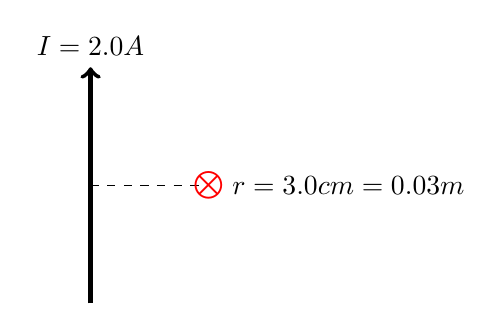
\begin{tikzpicture}
        \draw[ultra thick,->] (0,0) -- ++(0,3) node[above] {$I=\SI{2.0}{A}$};
        \draw[dashed] (0,1.5) -- ++(1.5,0); 
        \draw[red] (1.5,1.5) node {$\bigotimes$}  node[black,right=5pt] {$r = \SI{3.0}{cm} = \SI{0.03}{m}$};
    \end{tikzpicture}
\end{center}

We are given current and distance: $I=\SI{2.0}{A}$ and $r = \SI{3.0}{cm} = \SI{0.03}{m}$. \textbf{NOTE}: We must convert centimeters (cm) to meters (m). We know mu-zero is $\mymu_0 = 4\pi \times 10^{-7}$ and $\pi \approx 3.14$. Therefore, the magnitude of the magnetic field is, by Equation \ref{bJjNpw},

\begin{equation*}
    B=\frac{\mymu_0 I}{2\pi r} = \frac{\left(4\pi \times 10^{-7}\right)(2.0)}{2 \pi (0.03)} = \SI{1.3e-5}{T}
\end{equation*}

Therefore, 3 centimeters outside the wire, the magnetic field strength is \num{1.3e-5} tesla.

\vspace{1em}

\cyanhrule


\begin{mdframed}[backgroundcolor=black!10]
    \textbf{TIP}: When first learning these exercises, it's helpful to first try the calculations on Demos at \href{https://www.desmos.com/scientific}{desmos.com/scientific}. After, try replicating the calculations on a classroom calculator.
\end{mdframed}

\begin{example}
The magnetic field strength at some distance outside a wire that carries 4.9 amperes of current is \num{7.0e-7} tesla. Calculate this distance outside the wire.
\end{example}

\Solution We are given current and magnetic field: $I = \SI{4.9}{A}$ and $B = \SI{7.0e-7}{T}$. The unknown is distance: $r =\ ?$ These quantities are related by Equation \ref{bJjNpw}:

\begin{equation*}
    B = \frac{\mymu_0 I}{2\pi r}
\end{equation*}

Substituting the given values leads to 

\begin{equation*}
    \num{7.0e-7} = \frac{\left(4\pi \times 10^{-7}\right) (4.9)}{2\pi r}
\end{equation*}

We can solve this equation for $r$ as follows:

\begin{align*}
    \textbf{Cancel $\pi$} \qquad &  \num{7.0e-7} = \frac{\left(4\cancel{\pi} \times 10^{-7}\right) (4.9)}{2\cancel{\pi} r}\\[1ex]
    \textbf{Multiply by $r$} \qquad & \left(\num{7.0e-7}\right) \textcolor{red}{r} = \frac{\left(4 \times 10^{-7}\right) (4.9)}{2\cancel{r}} \redtimes \textcolor{red}{\cancel{r}}\\[1ex]
    \textbf{Compute 4/2 \& Simplify} \qquad & \left(\num{7.0e-7}\right) r = \left(\num{2e-7}\right) (4.9)\\[1ex]
    \textbf{Divide \num{7.0e-7}} \qquad & \frac{\left(\cancel{\num{7.0e-7}}\right) r}{\textcolor{red}{\cancel{\num{7.0e-7}}}} = \frac{\left(\num{2e-7}\right) (4.9)}{\textcolor{red}{\num{7.0e-7}}}\\[1ex]
    \textbf{Simplify} \qquad & r = \SI{1.4}{m}
\end{align*}

Therefore, the distance outside the wire is 1.4 meters.

\vspace{1em}

\cyanhrule

\clearpage

\subsection*{\ref{NErSiN} Exercises}

\begin{exercise}
    Identify the mathematical symbol for magnetic field.
\end{exercise}

\begin{exercise}
    What is the SI unit of magnetic field?
\end{exercise}


\begin{exercise}
    Write the constant $\mymu_0$ entirely numerically by computing the factor $4\pi$ numerically. (\textit{Hint}: typing \texttt{pi} into \href{https://www.desmos.com/scientific}{Desmos} translates to $\pi = 3.14159\ldots$ )
\end{exercise}

\begin{exercise}
    What does $I$ mean? What are its units?
\end{exercise}

\begin{exercise} \label{eibN4h}
    The electric current through a straight wire is \SI{2.4}{A}. What is the magnitude of the magnetic field at a point \SI{16}{cm} outside the wire?
\end{exercise}

\begin{exercise} \label{Z3KU8j}
    A magnetic field of \num{2.1e-5} tesla is measured at some distance outside a large wire carrying a strong current of 45 amperes. Calculate that distance outside the wire.
\end{exercise}

\begin{exercise} \label{toCeii}
    Calculate the magnetic field at the point shown below.

\begin{center}
    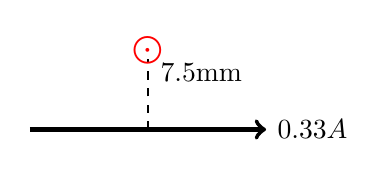
\begin{tikzpicture}
        \draw[ultra thick,->] (0,0) -- (3,0) node[right] {$\SI{0.33}{A}$};
        \draw[dashed] (1.5,0) -- ++(0,0.9);
        \node[red] at (1.5,1) {$\bigodot$};
        \node[below right=1pt] at (1.5,1) {\SI{7.5}{mm}};
    \end{tikzpicture}
\end{center}
\end{exercise}

\begin{exercise} \label{zCT6A5}
    The magnetic field strength 0.631 meters outside a current-carrying wire is \SI{3.49e-5}{T}. Calculate the electric current through the wire.
\end{exercise}

\begin{exercise}
    Solve Equation \ref{bJjNpw} for distance, $r$. Check that this new equation gives the same answer you got for Exercise \ref{Z3KU8j}. 
\end{exercise}

\begin{exercise}
    Solve Equation \ref{bJjNpw} for current, $I$. Check that this new equation gives the same answer you got for Exercise \ref{zCT6A5}. 
\end{exercise}

\begin{exercise}
    Why do you think $\pi$ appears in Equation \ref{bJjNpw}?
\end{exercise}

\begin{exercise}
A straight wire makes a \textit{curled} magnetic field. Do you think it's possible to make a \textit{straight} magnetic field? How?
\end{exercise}

\clearpage

\subsection*{Answers to Select Exercises}

\ref{eibN4h}. \SI{3.0e-6}{T}\\
\ref{Z3KU8j}. \SI{0.43}{m}\\
\ref{toCeii}. \SI{8.8e-6}{T}\\
\ref{zCT6A5}. \SI{110}{A}\\



\subsection*{Additional Resources}

\begin{itemize}
    \item \textit{YouTube}: ``Magnetic Torpedoes'' by \texttt{Grand Illusions} (\href{https://youtu.be/jbGaSL6wJ8M}{click here})
    \item \textit{YouTube}: ``Cool Experiment Sand, Magnet \& Iron filings'' by \texttt{Lifehacker \& Experimenter} (\href{https://youtu.be/tfiebTsJDno}{click here})
    \item \textit{PhET Simulation}: ``Magnet and Compass'' (\href{https://phet.colorado.edu/en/simulation/legacy/magnet-and-compass}{click here})
\end{itemize}




\clearpage
\printnoidxglossaries

\end{document}


\documentclass{article}
\usepackage{preamble}
\setlength{\parskip}{1em}



\title{Chapter 20: Magnetism}
\author{}
\date{}



\begin{document}


\end{document}